\subsection{Data poisoning}

Data poisoning occurs when the training of the neural network has been performed with incorrect data. The adversary has deliberately planted/altered information to be used in training such that most of the time the trained network would perform as expected, but there will be specific cases where the network classifies wrongly.

Online training based on samples submitted by others are particularly vulnerable to this type of attack. For example Google has an online game called `Quick, Draw!' which classifies doodles drawn by the players. The players are given an object to draw, the neural network then tries to classify the doodle as it is being drawn. After the game ends, the doodles drawn are then added to the training set of the network. If an adversary deliberately draws a circle every time a square is asked for, then this will result in changes of the network parameters and may cause future misclassifications. 

This type of attack is also a worry if the training has been outsourced. How can you tell if the neural network has been trained on the correct data?

\begin{figure}[h!] 
	\centering
	\begin{subfigure}{.4\textwidth}
		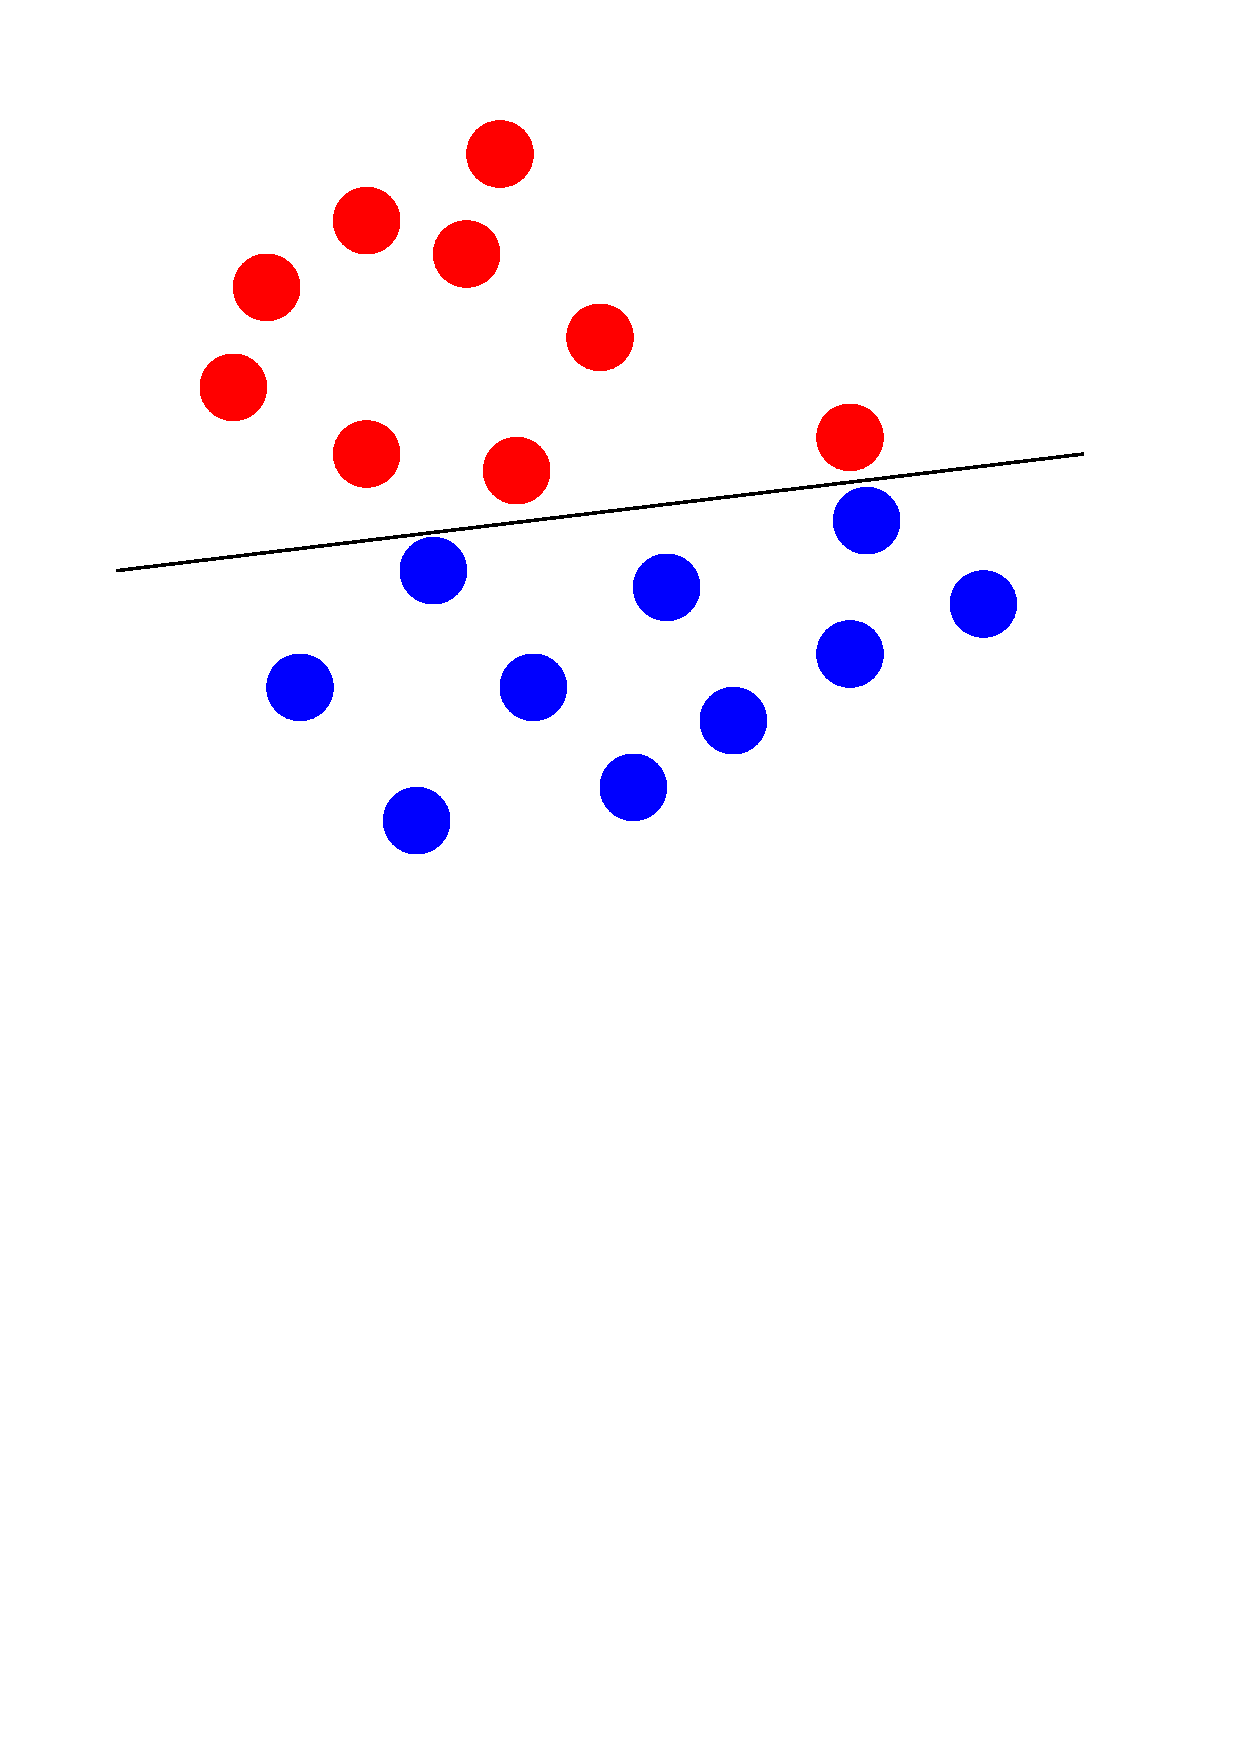
\includegraphics[width=\textwidth]{original}
		\caption{The original data}
		\label{fig:original}
	\end{subfigure}
	\begin{subfigure}{.4\textwidth}
		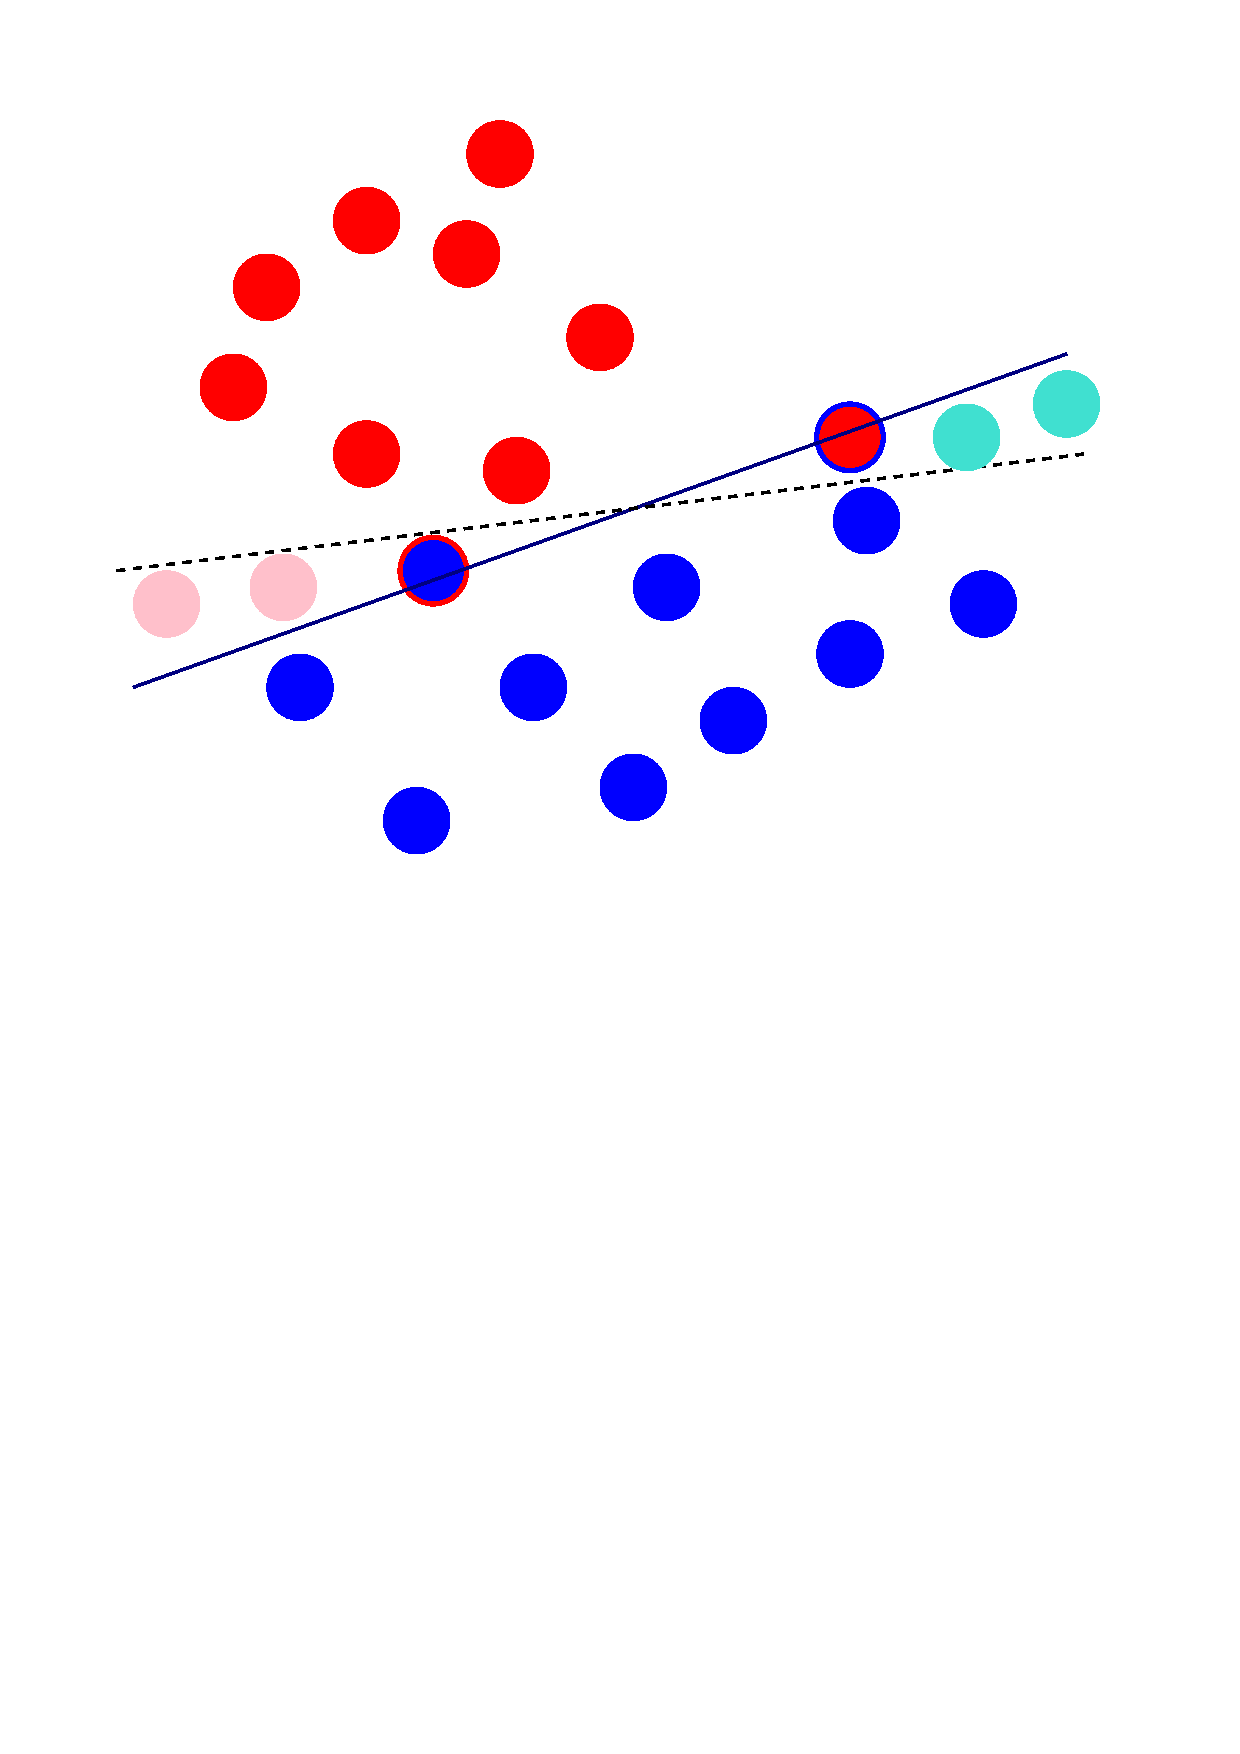
\includegraphics[width=\textwidth]{data_poisoning}
		\caption{Our model}
		\label{fig:poison}
	\end{subfigure}
	\caption{With data poisoning}
	\label{fig:poisoning}
\end{figure}

We can see a representation of this concept in Figure \ref{fig:poisoning}. On the left we have the unattacked system, on the right additional pink points and turquoise points (these are spurious data for the red and blue class respectively) have been used to train the network. This has led to the classification boundaries to change from the dashed line to the solid line, and as a result a blue point and a red point would be misclassified.
